\chapter{Einleitung}
\label{cha:Einleitung}

\section{Ziel der Arbeit anhand eines Beispiels} 
\label{sec:ZielDerArbeit}
\begin{figure}[htb]
\centering
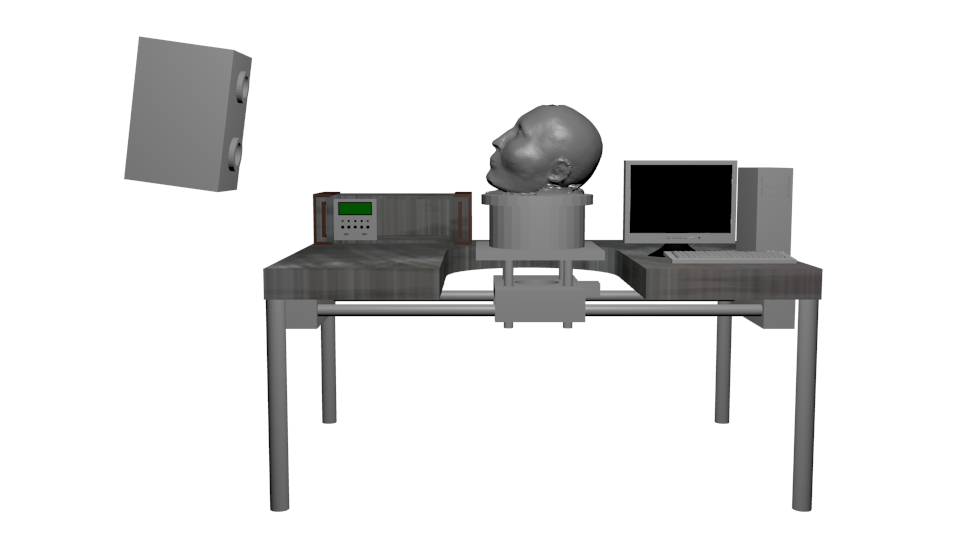
\includegraphics[width=\textwidth]{Blender/Schema_Arbeitsplatz.png}
\caption{Blick auf den Arbeitsaufbau}
\label{fig:Übersicht}
\end{figure}

\subsection{Vorhandene Komponenten}
\begin{enumerate}
\item Computer mit Erfassungssoftware RapidForm2004
\item 3D-Laserscanner VI-900
\item Arbeitstisch mit integriertem Drehtisch
\item 19''-Rack mit 2 Schrittmotorkarten
\item Mikrocontroller
\end{enumerate}
\subsection{Vorgaben}
Aufbau eines Übersetzers, basierend auf einem Mikrocontroller. Der Übersetzer sollte ein LC-Display, mehrere Taster, mehrere LEDs und zwei serielle Schnittstellen enthalten. Die Höhenverstellung des Drehtisches sollte genutzt werden und die zu Beginn noch nicht funktionierenden Endschalter sollten die vorgesehene Funktion erfüllen.\\ Im konkreten Beispiel ging es um die automatische 3D-Erfassung eines Schädelmodells. In der Ausgangssituation war es zwar möglich, mit der Erfassungssoftware RapidForm2004 und dem 3D-Laserscanner VI-900  einen Schädel aus einer Richtung zu erfassen. Die Kommunikation zwischen dem VI-900 und der Erfassungssoftware funktionierte. Die Drehtischsteuerung, welche den Drehtisch nach den Vorgaben der Erfassungssoftware des Computers drehen sollte, war nicht in das System eingebunden. Dies war ein Problem der verschiedenen Befehlssätze.
\subsection{Zielvorgabe}
\begin{enumerate}
\item Der VI-900 erstellt eine Aufnahme des Schädels.
\item Der VI-900 sendet die Aufnahme an die Erfassungssoftware im Computer.
\item Die Erfassungssoftware im Computer sendet nach der Speicherung der Aufnahme den Befehl zum Drehen des Drehtisches an die Drehtischsteuerung.
\item Die Drehtischsteuerung dreht den Tisch um die gewünschte Gradzahl.
\item Die Drehtischsteuerung meldet die erfolgreiche Rotation mit Hilfe des zu entwickelnden Übersetzers an die Erfassungssoftware im Computer.
\item Die Erfassungssoftware im Computer sendet erneut einen Aufnahmebefehl an den VI-900.
\end{enumerate}
Nachdem ein kompletter Aufnahmesatz im Computer eingespeichert ist, kann das 3D-Modell als CAD-Datei exportiert werden.
Das Erstellen eines kompletten Aufnahmesatzes soll auch für Laien leicht möglich sein.

\section{Motivation}
\label{sec:Motivation}
Die 3D-Lasererfassung bietet zahlreiche Anwendungsgebiete. 
\begin{itemize}
\item Qualitätskontrolle und Bauteilprüfung für Guss- und Spritzgusstechnik
\item Erstellung von Finite-Elemente-Daten für Blechteile im Karosseriebau usw. in Verbindung mit Bauteilanalyse
\item Erstellung von 3D-Daten zur Kontrolle von Zubehörteilen und anderen Zukaufteilen, für die keine 3D-CAD-Daten verfügbar sind (z.B. Reverse Engineering)
\item Umwandlung von Daten aus der Zahnmedizin und der plastischen Chirurgie in ein Datenbankformat
\item Erstellen von Konstruktionsdaten aus Mustern und Verzugs-Prüfung an mechanischen Bauteilen
\item Integration in Rapid-Prototyping-Systemen für die Erstellung von Mustern aus Kunststoff
\item Vergleich von Eigenprodukten mit Produkten des Mitbewerbs und Umwandlung der erfassten Daten in ein Datenbankformat
\item Archivierung in Museen und Forschungseinrichtungen
\item Erstellung von Daten für die CAE-Analyse
\item 3D-Daten von beliebigen Objekten für unterschiedlichste Forschungszwecke
\item Informations- und Kommunikationstechnik, Mimikanalyse, Muskelbewegungsanalyse, Robot-Vision und Wachstumskontrolle landwirtschaftlicher Erzeugnisse
\item Unterschiedliche Anwendungen in der Filmindustrie
\end{itemize}\cite{Minolta:Einleitung}
Im konkreten Fall soll nun die Erstellung von 3D-Daten eines vorhanden Objektes (\Fachbegriff{Reverse Engineering}) genutzt werden.\\
Es wird nun mit einer Kombination aus dem 3D-Laserscanner, dem Drehtisch und der dazugehörigen Erfassungssoftware ein 3D-Modell erfasst. Dieses kann dann unterstützend in der \Fachbegriff{CAD-Entwicklung} genutzt werden kann.\\
In der CAD-Entwicklung kann es vorkommen das für ein real existierendes Objekt eine \textit{Erweiterung} konstruiert werden soll. Um die Erweiterung, einen Anschlag zum Beispiel, leichter konstruieren zu können, ist es von Vorteil, die Abmessungen des Objektes möglichst genau zu kennen. Das Übertragen der Abmessungen in die CAD-Software kann, insbesondere für komplexe Objekte, sehr aufwendig sein.
Abhilfe soll der 3D-Laserscanner schaffen, der das Objekt aus mehreren Richtungen vermisst und aus diesen Informationen ein 3D-Modell generiert. Dieses soll dann in einem neutralen CAD-Format \todo{welches?} exportiert werden.